\frame{
    \frametitle{The radius function}
    \begin{block}{Neighborhood function $\Theta$: the radius $\sigma$}
        \begin{equation*}
            \Theta(t,\beta_{1},\beta_{2})=\exp\left(-\frac{(i-\beta_{1})^{2}+(j-\beta_{2})^{2}}{2\sigma^{2}(t)}\right)
        \end{equation*}
        \begin{columns}
            \begin{column}{0.4\textwidth}
                $\sigma = 1.7$\\
                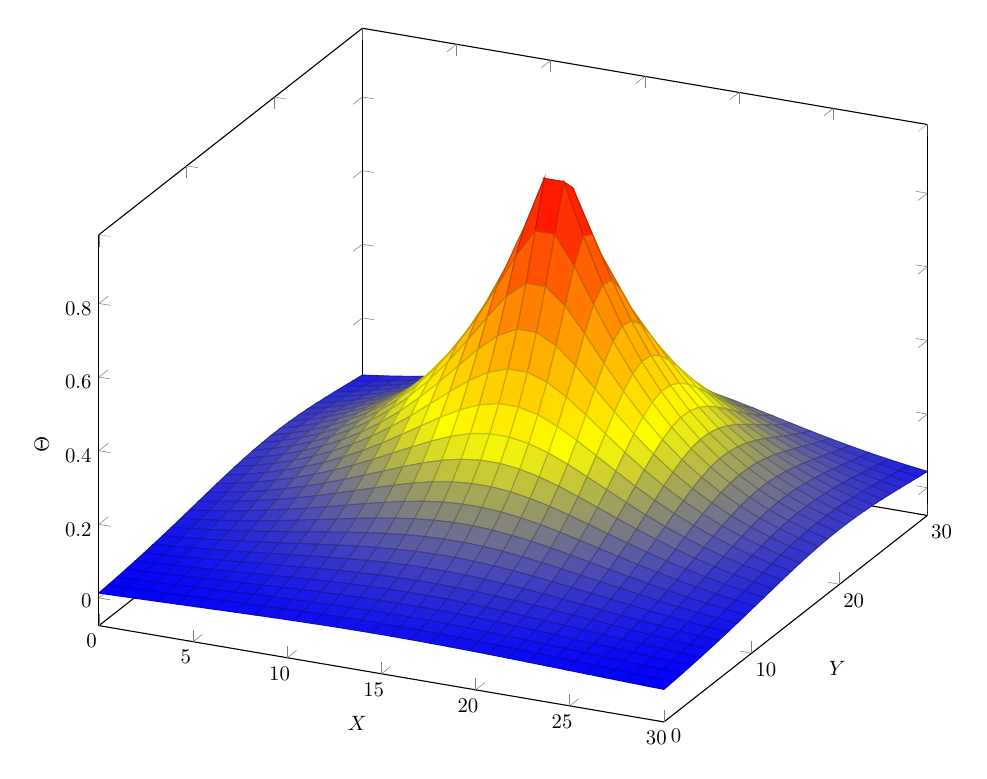
\begin{tikzpicture}[scale=1, every node/.style={scale=0.75}]
                    \pgfplotsset{width=\textwidth,compat=1.3}
                          \begin{axis}[xlabel=$X$, ylabel=$Y$,zlabel=$\Theta$]
                          \addplot3[surf,shader=faceted,domain=0:30,samples=30]
                              {exp( -1 * ( sqrt((x-15)^2+(y-20)^2)/(2*1.7^2) ) )};
                         \end{axis}
                \end{tikzpicture}
            \end{column}
            \begin{column}{0.4\textwidth}
                $\sigma=1$\\
                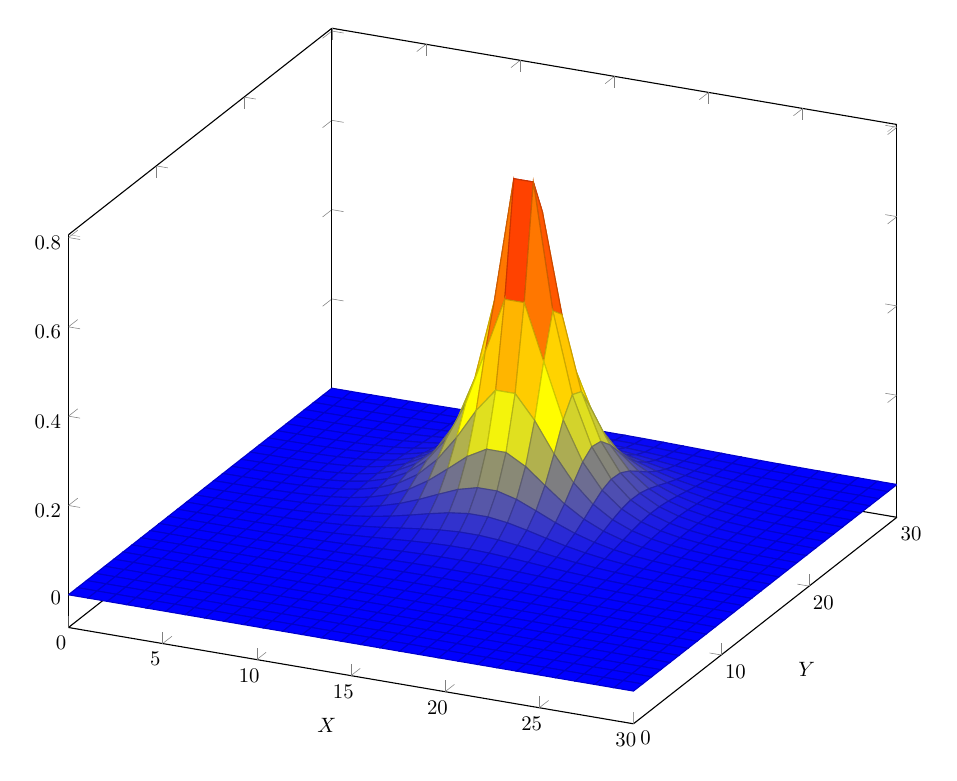
\begin{tikzpicture}[scale=1, every node/.style={scale=0.75}]
                    \pgfplotsset{width=\textwidth,compat=1.3}
                          \begin{axis}[xlabel=$X$, ylabel=$Y$]
                          \addplot3[surf,shader=faceted,domain=0:30,samples=30]
                              {exp( -1 * ( sqrt((x-15)^2+(y-20)^2)/(2*1^2) ) )};
                         \end{axis}
                \end{tikzpicture}
            \end{column}
        \end{columns}
        \begin{equation*}
            \sigma(t)=(\sigma(t_{i})-\sigma(t_{f}))\cdot\exp(-\frac{t}{\lambda})+\sigma(t_{f})
        \end{equation*}
    \end{block}
}
